% !TeX root = ../main.tex

\section{处理函数}

\subsection{区分函数和局部变量}

编译器前端生成的语法树,在没有进行语义分析之前,
没有也无法区分函数名和变量名。
但是对于访问函数,无论是直接调用还是将其赋值给其他变量,
我们需要将其翻译成 leaq 指令,这和访问变量是不同的。
因此我们需要区分开来函数名和变量名。

由于我们已经进行了标识符唯一化,这个工作就变得非常简单。
就像处理可变变量那样,我们引入 Funref 结构体,
把所有出现的使用全局定义的函数名的地方,全部换成 Funref 语句即可。
后面翻译为 x86 时再将其翻译为 leaq 指令。
例如:

\begin{transformation}
\begin{lstlisting}
(define (f) : Integer
  ...)
(let ([g f])
  g)
\end{lstlisting}
\compilesto
\begin{lstlisting}
(define (f) : Integer
  ...)
(let ([g (Funref f)])
  g)
\end{lstlisting}
\end{transformation}

\subsection{生成闭包}

如果一个变量出现在 e 中,但在 e 中没有定义,
那么就称该变量在表达式 e 中是“自由变量”。

例如,在下面的表达式中,x 和 y 为自由变量。
\begin{lstlisting}
  (lambda: ([z : Integer]) : Integer
    (+ x y z))
\end{lstlisting}

而闭包则是引用了自由变量的函数,被引用的自由变量和函数一同存在,
即使已经离开了自由变量的环境也不会被释放或者删除,在闭包中可以继续使用这个自由变量。

例如:
\begin{lstlisting}
  (define (f [x : Integer]) : (Integer -> Integer)
    (let ([y 4])
      (lambda: ([z : Integer]) : Integer
        (+ x y z))))

  (let ([g (f 5)])
    (let ([h (f 3)])
      (+ (g 11) (h 15))))
\end{lstlisting}

f 接受一个参数 x,在其内部创建一个值为 4 的局部变量 y,然后返回一个匿名函数。
这个匿名函数接受一个参数 z,返回 \code{x+y+z} 的值。
对于这个 lambda 表达式,x 和 y 是自由变量。

接下来是两次对 f 的调用,参数 x 分别被传入了 3 和 5。
从 f 返回的匿名函数被绑定到变量 g 和 h。
尽管这两个函数是由同一个 lambda 创建的,但它们实际上是不同的函数,
因为g 和 h 中 x 的值显然不同。
然后,调用\code{(g 11)}会执行\code{(+ 5 4 11)},
调用\code{(h 15)}会执行\code{(+ 3 4 15)},二者相加最终得到 42。
显然,在调用g 和 h时,我们需要某种方法来读取到正确的 x 和 y 的值。

我们的解决方法是在每次调用函数时,把自由变量的值与函数指针放到一个向量中,
并把这个向量作为额外的参数传入进去。
这个技术称作扁平闭包\cite{Cardelli_1983},通常直接就称为闭包。
我们看一下在上面的例子中,闭包是如何工作的。

首先,匿名函数也是函数,编译成汇编代码后它们同样是从一个标签开始的一段指令。
因此,所有匿名函数都会被提出来变成全局函数,并赋予它们新的函数名。

程序首先调用函数 f ,它为 lambda 创建一个闭包。
闭包其实就是一个向量(元组),它的第一个元素是一个指针,指向我们将为 lambda 生成的顶级函数,
第二个元素是 x 的值,即 5,第三个元素是 4 ,即 y 的值。
闭包中不包含 z,因为 z 不是 lambda 的自由变量。创建结束是第一步。
闭包从 f 返回并绑定到 g ,如图\ref{fig:closure-eg}所示。
对 f 的第二次调用创建另一个闭包,这一次闭包的第二个元素是 3。
这个闭包也从 f 返回,但绑定到 h ,如图\ref{fig:closure-eg}所示。

接下来考虑\code{(g 11)}。
要调用闭包,我们拿到闭包第一个元素中的函数指针并调用它,
传入闭包本身,然后传入常规参数,也就是 11。

最后,我们还要为 lambda 生成顶层函数。
这个顶层函数会多出一个参数,用来接受闭包。
然后对于每个自由变量,我们要在函数的开头从闭包中取出这些自由变量的值,
绑定到这些自由变量上。这一步称为闭包转换。

图\ref{fig:colure-conversion-eg}展示了这个例子的转换结果。
注意,虽然 f 函数本身就是全局定义的函数,它的函数体里没有任何自由变量,
我们还是给它添加了一个额外的参数用以接受闭包。
这样一来,我们就可以统一对待从匿名函数提取出来的全局函数和原本的全局函数,
不需要再在后续的翻译工作中区分它们。

我们使用了一条下划线来表示闭包的类型,下划线表明我们不在意这个变量的类型,
也不需要对其进行类型检查。
之所以可以这么做是因为闭包是由编译器生成的,
我们的转换代码可以保证我们总是能正确的使用这些闭包变量。
而之所以要这么做是因为本文现有的类型系统无法正确地表示闭包的类型
\footnote{正确描述闭包的类型需要使用存在类型\cite{Minamide_Morrisett_Harper_1996}。}
:闭包中的元素间接指向了闭包自己——
第一个元素是函数,而这个函数又接受这个闭包作为第一个参数。

\begin{figure}[t]
\centering 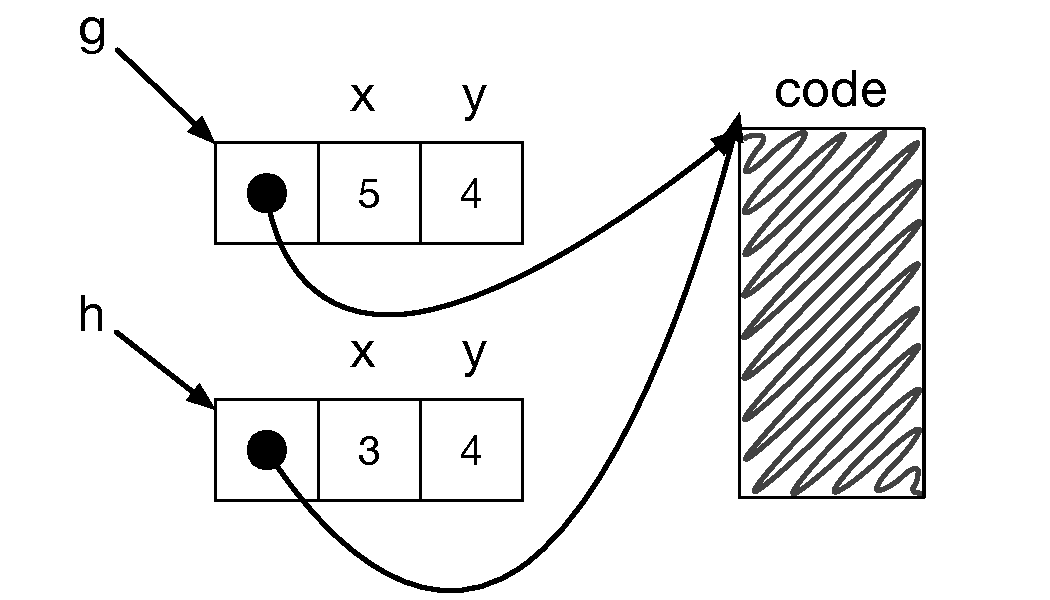
\includegraphics[width=0.6\textwidth]{figures/closures}
\caption{闭包示意图}
\label{fig:closure-eg}
\end{figure}

\begin{figure}[tbp]
  \begin{minipage}{0.8\textwidth}
% tests/lambda_test_6.rkt
\begin{lstlisting}[basicstyle=\ttfamily\footnotesize]
(define (f [x : Integer]) : (Integer -> Integer)
  (let ([y 4])
    (lambda: ([z : Integer]) : Integer
      (+ x (+ y z)))))

(define (main) : Integer
  (let ([g ((fun-ref f) 5)])
    (let ([h ((fun-ref f) 3)])
      (+ (g 11) (h 15)))))
\end{lstlisting}
$\Rightarrow$
\begin{lstlisting}[basicstyle=\ttfamily\footnotesize]
(define (f [clos2 : _] [x : Integer]) : (Vector ((Vector _) Integer -> Integer))
  (let ([y 4])
    (vector (list (fun-ref lambda2) x y))))

(define (lambda2 [clos3 : (Vector _ Integer Integer)] [z : Integer]) : Integer
  (let ([x (vector-ref clos3 1)])
    (let ([y (vector-ref clos3 2)])
      (+ x (+ y z)))))

(define (main) : Integer
  (let ([g (let ([clos5 (vector (list (fun-ref f6)))])
             ((vector-ref clos5 0) clos5 5))])
    (let ([h (let ([clos6 (vector (list (fun-ref f6)))])
               ((vector-ref clos6 0) clos6 3))])
      (+ ((vector-ref g 0) g 11) ((vector-ref h 0) h 15)))))
\end{lstlisting}
\end{minipage}

\caption{闭包转换示例}
\label{fig:colure-conversion-eg}
\end{figure}


\subsection{赋值对闭包的影响}

考虑下面这个例子:

\begin{lstlisting}
  (define (f) : (-> Integer)
    (let ([x 0])
      (let ([g (lambda: () : Integer x)])
        (begin
          (set! x 42)
          g))))
  ((f))
\end{lstlisting}

函数 f 中定义了局部变量 x,初始值为0。
然后定义了一个无参匿名函数,函数体只有一个表达式 x。
也就是它什么都不做,直接返回 x。
接着我们把 x 的值改为 42,然后返回刚才的匿名函数。
我们期望\code{((f))}的返回值是 42。

但是上一小节描述的闭包转换会把正在编译闭包时x的值,也就是 0,放入闭包中。
这样编译出来的程序就会返回错误的结果 0。

并且,虽然x是函数f的局部变量,它的生命周期却超过了 f的生命周期。
这说明了自由变量的生命周期是不确定的。
在这个例子中,函数f执行结束后就退出了,但局部变量 x 仍然需要被匿名函数访问。
只有当这个匿名函数也无法被访问到时,我们才可以放心地清理掉变量 x。
因此,自由变量的值需要存放在堆上。
我们通常使用“box”来表示这种在堆上分配单个值的行为,“unbox”则指代对box的解引用。
这里我们并不需要引入 box 结构,单元素的向量就是box。

虽然理论上来说自由变量的生命周期是不确定的,但并非所有的自由变量我们都要放在堆上。
对于那些在代码中只有定义,没有重新被赋值的变量,
我们还是可以简单地把它们的值放在闭包中。
由于box会引入额外的开销,因此在本文的实现中,
只有那些可能被重新赋值的(也就是在代码中出现在\code{set!}语句中的)自由变量才会被box。
上面例子中的f函数,在转换后将得到以下结果。

\begin{lstlisting}
(define (f) : (-> Integer)
  (let ([x (vector 0)])
    (let ([g (lambda: () : Integer
               (vector-ref x 0))])
      (begin
        (vector-set! x 0 42)
        g))))
\end{lstlisting}
